\section{Philosophie de CRUSH}

\begin{PimpedBox}
Un des enjeux majeurs des systèmes de stockage distribué consiste d'une part à répartir de manière efficace, redondante et rapide une quantité importante de données sur plusieurs disques -- des centaines voire des milliers -- et d'autre part à être capable de récupérer cette information de manière tout aussi fiable, rapide et sans goulot d'étranglement.
\end{PimpedBox}

Comme expliqué précédemment, CEPH a par ailleurs pour vocation d'être évolutif en termes de capacité de stockage (\textit{scalable}). Ceci pose donc une contrainte d'utilisation des disques ; dans une base de données classique, les disques dernièrement ajoutés, souvent plus performants, ne sont que très peu utilisés tandis que les anciens disques ont été remplis au fur et à mesure et sont donc utilisés au maximum de leur capacités. Cette contrainte est d'autant plus forte que les vieux disques auront statistiquement plus de chance d'avoir une panne que les nouveaux. 

Par ailleurs, CEPH veut s'abstraire au maximum des machines physiques pour ne pas dépendre d'un système spécifique de machines et accepter toutes sortes d'architectures.

Pour adresser ces différentes contraintes, CEPH s'appuie sur un algorithme spécifique nommé \textbf{CRUSH}. Cet algorithme est une implémentation spécifique des algorithmes de type \textbf{RUSH}\footnote{Les algorithmes RUSH tentent de répondre à la problématique de répartition uniforme des données dans un large panel de disque pour répartir la charge d'utilisation.} et permet en effet d'apporter de nouvelles réponses à ces problématiques. Ainsi, CRUSH est un algorithme \textbf{pseudo-aléatoire}\footnote{Ce terme est employé pour des raisons de simplicité, et le caractère \og{}pseudo-aléatoire\fg{} de CRUSH est affiné par la suite.} de répartition des données, c'est-à-dire qu'il va répartir les données de manière uniforme sur l'ensemble des disques. Si la répartition des données semble donc aléatoire, CRUSH reste un algorithme \textbf{déterministe}. À contexte égal, la réponse à une entrée restera toujours la même, quel que soit le nombre d'exécutions de l'algorithme. En ce sens, CRUSH peut être \textit{imaginé} comme la rencontre d'une fonction pseudo-aléatoire et d'une fonction de hachage.

Pour mener à bien cette répartition, CRUSH utilise une carte du cluster, ou \textit{cluster map}. Cette carte est définie par l'administrateur et permet de spécifier l'état du système sur un grand nombre de paramètres. Elle comporte en effet une représentation sous forme d'arbre ou chaque feuille (\textit{device}) indique le nombre de réplicats nécessaires. Chaque nœud (\textit{bucket}) peut être lié à d'autres selon qu'il partage des points de défaillance communs, comme une même source d'alimentation ou un même réseau.

Par ailleurs, CRUSH peut mettre à jour sa carte sans réorganiser la totalité de ses données. L'algorithme répond à des objectifs de \textbf{minimisation} des déplacements inutiles des données et de scalabilité. Ainsi, lorsqu'un nouveau disque est ajouté, des données sont aléatoirement migrées sur le nouveau disque, créant un équilibre et permettant une meilleure répartition du travail dans le cluster et donc des performances accrues. Il va cependant déplacer bien moins de données qu'un algorithme de hachage classique qui nécessite bien souvent une complète réorganisation des données. 

\begin{PimpedBox}
CRUSH se comporte comme une fonction de hachage, sauf lorsque la carte du cluster est modifié. Dans ce cas, certaines données sont déplacées de manière à homogénéiser le stockage, mais la plupart des données restent où elles sont. C'est ce qui le différencie d'une part de l'aléatoire et d'autre part du hachage.
\end{PimpedBox}

\newpage
Trois avantages majeurs se dégagent donc :

\begin{itemize}
\item Chaque partie du système peut calculer l'emplacement d'un objet en ne connaissant que la carte du cluster et les règles de placement, ou \textit{placement rules}.
\item Une moindre dépendance vis-à-vis des métadonnées, CRUSH se basant plus sur des fonctions déterministes afin de déterminer l'emplacement des données à écrire ou lire.
\item Une réorganisation minimale en cas de modification de l'architecture.
\end{itemize}

\section{Carte du cluster}

Dans l'algorithme CRUSH, la distribution des données est contrôlée par une carte du cluster hiérarchique, rendant compte à la fois des ressources de stockage disponibles et des éléments logiques organisant le système.

Grâce à la cluster map, l'administrateur va pouvoir rendre compte dans l'algorithme des contraintes organisationnelles de son serveur : par exemple, il pourra tout à fait regrouper les différents disques utilisant le même réseau électrique ou internet afin d'optimiser la réplication des données sur des réseaux différents.

La cluster map est composée d'une liste de \textit{devices} et de \textit{buckets} : à ces deux éléments on associe un \textbf{identifiant} et un \textbf{poids}.

Les buckets permettent de définir une arborescence au sein du système et de rendre compte des contraintes matérielles de l’installation : ils contiennent des devices et peuvent contenir d’autres buckets.

Le poids est, dans le cas d’un device, assigné par l'administrateur pour contrôler le nombre de données dont il est responsable : il est en lien avec la capacité du disque. À l'inverse, dans le cas d’un bucket, le poids correspond à la somme des poids des device et des buckets qui le composent.

CRUSH se base sur quatre types de buckets différents (voir section \ref{sssec:bucket}), chacun fonctionnant avec un algorithme de sélection différent pour traiter le mouvement des données.

\section{Règles de placement}

En rendant compte de  l'architecture du système par le biais de la cluster map, CRUSH peut modéliser et, par conséquent, résoudre les éventuelles sources de défaillances liées à l'organisation générale du système. 

Les sources de ces défaillances peuvent être variées : la proximité physique, une source d'alimentation partagée, réseau internet partagé etc.
En encodant ces informations dans la cluster map, les placement rules vont permettre de discriminer la réplication des données sur différents domaines d'échec, tout en conservant la distribution souhaitée.

Ces règles sont définies par l'administrateur, et permettent de contrôler de manière précise la politique de réplication des données au sein du système.

\section{Les différents types de bucket}
\label{sssec:bucket}

D'une manière générale, CRUSH est conçu pour concilier trois objectifs concurrents : efficacité, mise à l'échelle du mapping et minimisation des opérations de migration des données lors d'un ajout ou d'un retrait d'un disque du système. 

À cette fin, CRUSH définit quatre différents types de bucket, chacun impliquant l'utilisation d'une fonction différente pour le choix d'un item dans la hiérarchie (fonction $c(x,r)$ dans l'algorithme).

\begin{itemize}
\item \textbf{Uniform bucket} : ne peut contenir que des items de poids égaux.
\item \textbf{List bucket} : choisit l'item le plus récent possible, dont le poids dépasse la somme des poids des autres items dans le bucket.
\item \textbf{Tree bucket} : se rapproche dans le fonctionnement du bucket précédent, sauf qu'ici, les items sont représentés par des \textit{arbres binaires} de recherche.
\item \textbf{Straw bucket} : se base sur le jeu de la \textbf{courte paille}, en associant à chaque item du bucket une paille de longueur variable, lié au poids de l'item (un item plus lourd aura plus de chance de tirer une paille longue).
\end{itemize}

Le choix du bucket a une grande influence selon le type d'opération réalisée et la complexité de la fonction pseudo-aléatoire de sélection d'un item.
Ces considérations sont résumées dans le tableau \ref{chap3:tabBucket}.

\begin{table}
	\centering
  		\begin{tabular}{|c|c|c|c|c|}
           \hline
           \textbf{Action} & Uniform & List & Tree & Straw\\
           \hline
           \textbf{Complexité} & O(1) & O(n) & O(log n) &  O(n)  \\
           \hline
           \textbf{Ajout} & Mauvais & Optimal &  Bon & Optimal \\
           \hline
           \textbf{Suppression} & Mauvais & Mauvais &  Bon & Optimal \\
           \hline
  		\end{tabular}
        \caption{Résumé de la vitesse de mapping et de l'efficacité de la migration des données suit à l'ajout ou à la suppression d'un item, pour chaque type de \textit{bucket}.} \label{chap3:tabBucket}
\end{table}
\newpage

\section{Explication de l'algorithme}

À titre indicatif, l'algorithme complet est donné dans la figure \ref{chap3:CRUSH_algo} de l'annexe \ref{crush-algo}.

Pour stocker les données ou les retrouver -- il s'agit en fait de la même opération dans le cas de CRUSH --, l'algorithme est divisé en trois étapes. L'objet en question est un argument de l'algorithme ; nous le notons $x$.

\subsection{TAKE$(a)$}\label{chap3:take}
Cette fonction sélectionne un item $a$ (en général un bucket) contenu dans la hiérarchie de la carte du cluster et l'assigne au vecteur $\vec{i}$ : l'appel à cette fonction précède tout premier appel à la fonction \verb|SELECT| et peut être considéré comme la constitution de la racine, en ce sens où tous les autres éléments seront inclus dans cet item.

\subsection{SELECT$(n,t)$}
Cette fonction permet de déterminer un nombre d'items d'un certain type à partir de la sélection préalable (voir \ref{chap3:take}). Ces items constituent l'ensemble des \textbf{candidats} pour la réplication.

En particulier, elle itère sur chaque item $i \in \vec{i}$ et choisit $n$ éléments distincts de type $t$ dans la sous-arborescence de la racine courante au moment de l'appel à la fonction. Les devices et buckets ont en effet un type \textbf{fixé et connu}, ce qui permet le parcours de l'arborescence et la discrimination lors du choix des items, en fonction du type passé en argument.

Pour chaque $i \in \vec{i}$, la fonction va itérer sur $r \in (1,\ldots,n)$, $n$ correspondant au nombre d'items attendus, et va descendre récursivement dans tout bucket intermédiaire, en choisissant de manière pseudo-aléatoire un item dans chacun d'entre eux par le biais de la fonction $c(r,x)$, propre à chaque type de bucket -- jusqu'à trouver un item de type $t$.

Cependant, il se peut que tout ne se passe pas comme prévu, et ce pour plusieurs raisons: 

\begin{itemize}
\item Une collision peut arriver, \eg l'item choisi a déjà été choisi lors d'une précédente itération.
\item Le disque choisi est marqué comme \textit{failed} : erreur transitoire ou non.
\item Le disque choisi est marqué comme \textit{overloaded} : plus de mémoire.
\end{itemize}

Ces deux dernières erreurs sont envisageables car un disque peut être libellé comme \textit{failed} ou \textit{overloaded} dans la carte du cluster mais laissé dans la hiérarchie pour éviter les migrations de données inutiles.

Pour les périphériques \textit{failed} ou \textit{overloaded}, l'algorithme va redistribuer uniformément les éléments dans le système en redémarrant la récurrence au début de la fonction \verb|SELECT|.%(\textbf{repeat} ligne 11).

Dans le cas des collisions, un autre $r'$ est utilisé d'abord au niveau de la hiérarchie où la collision s'est déclarée, pour tenter une recherche locale.% (\textbf{repeat} ligne 14).

La fonction assigne finalement les $n$ items distincts de type $t$ au vecteur $\vec{i}$, qui peut soit être utilisé pour un nouvel appel à la fonction \verb|SELECT|, soit assigné au vecteur résultat $\vec{R}$ par le biais de l'appel à la fonction \verb|EMIT| (voir \ref{chap3:emit}).

\subsection{EMIT}\label{chap3:emit}

Cette fonction permet de constituer le vecteur résultat $\vec{R}$ à l'aide du vecteur $\vec{i}$.

\subsection{Gestion des erreurs}

En cas d'erreur, CRUSH utilise deux systèmes de remplacement en fonction du type de réplication (\textbf{totale} ou \textbf{partielle}, \ie par code correcteur). 

Dans les cas de réplication primaire, \ie l'objet est entièrement copié, si un des réplica subit une erreur CRUSH utilise un système dit de \og{}\textit{first n}\fg{}. En assignant $r' = r + f$, où $f$ est le nombre de placements échoués, les réplicas sont alors tous décalés \textbf{de $n$ positions} dans la liste.

À l'inverse, dans le cas d'une réplication partielle, CRUSH considère $r' = r + f_{r}n)$, où $f_{r}n$ est le nombre de tentatives échouées \textbf{sur $r$}. Ainsi, la séquence de candidats pour chaque réplica est indépendant des erreurs des autres.

La figure \ref{chap3:CRUSH_error} illustre ce comportement.

\begin{figure}
  \centering
  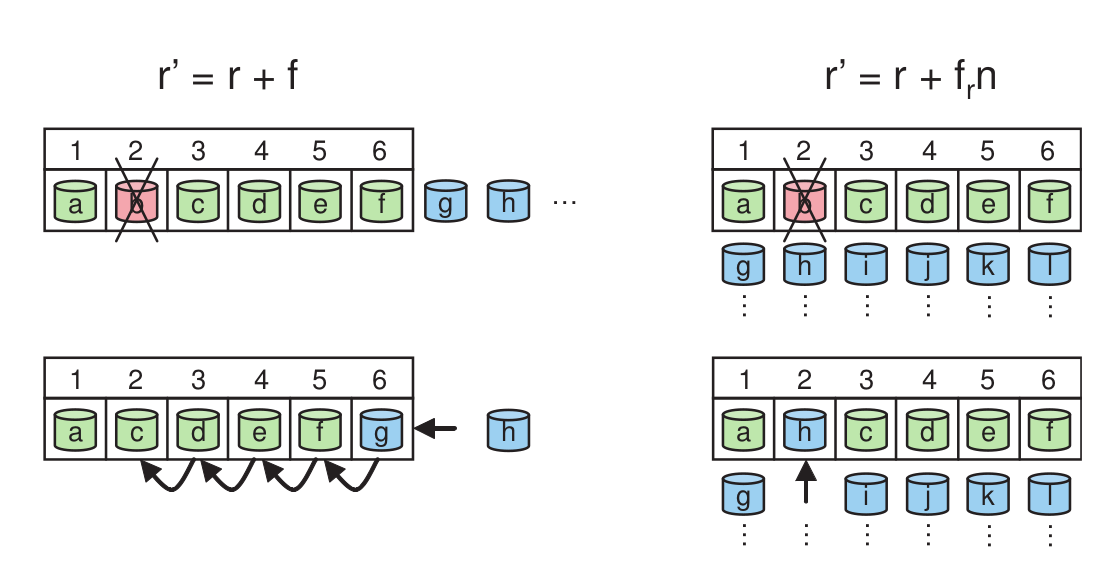
\includegraphics[scale=0.35]{./images/remplacement_erreur.png}
  \caption{Aperçu graphique de la gestion des erreurs dans CRUSH.}
  \label{chap3:CRUSH_error}
\end{figure}

\section{Exemple de résultat}

Considérons une cluster map composée de \textit{rows}, \textit{cabinets} et de \textit{disks} et les règles de placement indiquées dans le tableau \ref{chap3:tabPlacementRules}.

\begin{table}[htb]
	\centering
  		\begin{tabular}{|c|c|c|}
           \hline
           \textbf{n°} & \textbf{Action} & Vecteur $\vec{i}$\\
           \hline
           \textbf{1} & take(root) & root  \\
           \hline
           \textbf{2} & select(1, row) & row2 \\
           \hline
           \textbf{3} & select(3, cabinet) & cab21 cab23 cab24 \\
           \hline
           \textbf{4} & select(1, disk) & disk2107 disk2313 disk2437\\
           \hline
           \textbf{5} & emit & \\
           \hline
  		\end{tabular}
        \caption{Exemple de règles permettant d'obtenir 3 disques distincts, de trois \textit{cabinets} différents, dans un même \textit{row}. \label{chap3:tabPlacementRules}}
\end{table}

\begin{enumerate}
\item On sélectionne la racine à partir de laquelle on va effectuer la recherche (ici \textit{root}).
\item On sélectionne un item de type \textit{row} (ici \textit{row2}).
\item On sélectionne trois items de type \textit{cabinet}, inclus dans \textit{row2}, résultat du précédent appel à la fonction.
\item On itère sur les trois \textit{cabinets}, et on choisi un seul \textit{disk} contenu dans chacun d'eux.
\item On ajoute le résultat dans le vecteur $\vec{R}$.
\end{enumerate}

Finalement, on se retrouve avec trois \textit{disks}, éclatés dans trois \textit{bucket} distincts de type \textit{cabinet}, eux même inclus dans un \textit{bucket} de type \textit{row}.

La figure \ref{chap3:CRUSH_execution} montre une vue partielle de la hiérarchie définie par la cluster map. Les lignes en gras illustrent les items sélectionnés par chaque appel de \verb|SELECT|.

\begin{figure}[h]
    \centering
    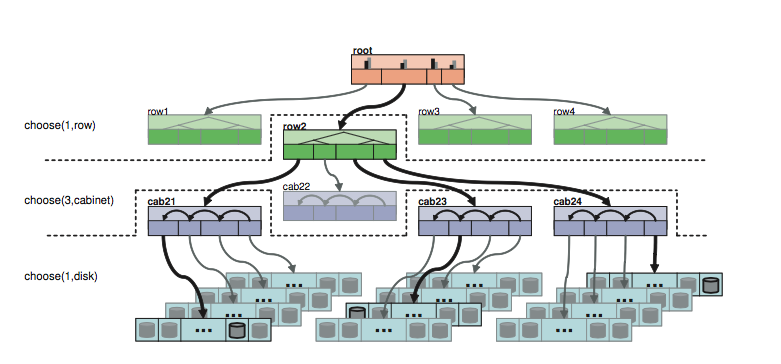
\includegraphics[scale=0.5]{./images/CRUSH_execution.png}
    \caption{Exemple de vue partielle de la sélection des items dans CRUSH.}
    \label{chap3:CRUSH_execution}
\end{figure}